\section{Experimental Results}
\label{Section:ExperimentalResults}

This section reports what the design of Section~\ref{Section:Implementation} produced. Seven agents were trained, one per major currency pair, and each was evaluated over eleven years under the cost model of Table~\ref{Tables:CostModel}. Every figure below traces to a stored run that can be reopened, and the analysis was recomputed from those runs rather than copied from the training logs.

The order of the section is deliberate. Returns come first, then the checks that decide whether those returns mean anything, then the year that was held back, and finally the result of running the seven together.

\subsection{Evaluation Protocol}
\label{Subsection:EvaluationProtocol}

The account, the cost model and the execution engine are described in Section~\ref{Subsection:TradingFramework} and are not repeated here. Three things are specific to the evaluation.

The window runs from 1 January 2015 to 1 January 2026, eleven years. It starts a year after the data begins so that the slowest indicator in the observation, a moving average over five thousand hourly bars, is fully warmed before the first decision.

Every result is measured from five different starting balances, of $9\,900$, $10\,000$, $10\,050$, $10\,100$ and $10\,200$ euros. A trading strategy that depends on its entry point is not a strategy, and small changes to the opening balance shift the rounding of every position size and therefore the whole sequence of trades. Reporting one balance would hide that sensitivity, so the tables give the mean across the five and the spread around it.

Position size is a per-pair parameter, chosen by the sweep described in Section~\ref{Subsection:ExperimentalProcedure} rather than fixed in advance. Five pairs use the reference risk of Equation~\ref{Equation:PositionSizing}, NZD/USD uses one and a half times it, and USD/JPY uses a smaller fraction of it. Position size scales the size of every trade but does not change the policy that chooses them, so the ratios, the alpha and beta decomposition and the correlation structure are all unaffected by it.

\subsection{Benchmarks and Performance Metrics}

The benchmark is buying the pair at the start of the window and holding it to the end. It is the honest comparison for a directional strategy on a single instrument: it is available to anyone, it costs one spread, and any strategy that cannot beat it has not earned its complexity. The proposal named a random-signal baseline and a moving-average crossover instead; both were dropped because neither is a strategy a trader would actually hold as an alternative.

The reported metrics are those defined in Section~\ref{Subsection:PerformanceMeasurement}: total and annualised return, the Sharpe, Sortino, Calmar and Sterling ratios, maximum drawdown and the number of trades. Table~\ref{Tables:PerformanceMetrics} states what each one measures. Ratios use a zero risk-free rate throughout, so they can be compared with each other across pairs without a rate assumption entering.

\input{Tables/PerformanceMetrics}

Four of them deserve a word on why they are all reported rather than one being chosen. Return says how much was made and nothing about the cost of making it. The Sharpe ratio divides return by total volatility, which penalises a strategy for moving upwards as much as for moving downwards. The Sortino ratio corrects that by counting only downside movement. Calmar and Sterling divide by drawdown instead of volatility, the first by the worst loss ever suffered and the second by the average one, so they answer the question an investor actually asks, which is how far the account fell rather than how much it wobbled. A strategy can look strong on one of these and weak on another, and where that happens in this work it is pointed out.

One point applies to every number in this section. Returns are net of the spread quoted at the moment of each trade and of the commission of the account in Table~\ref{Tables:CostModel}. They are therefore not comparable with results computed on bar closes with a fixed or absent spread, and they are lower than the same policies would show under those conditions.

\subsection{Results Across the Seven Majors}
\label{Subsection:PairResults}

Table~\ref{Tables:PairResults} gives the result for each pair, in alphabetical order. Total return over the eleven years ranges from $+226.6\%$ on USD/CAD, the strongest, to $+15.7\%$ on USD/JPY, the weakest. Every pair is profitable, and every pair is profitable from all five starting balances.

\begin{table}[htb!]
\centering
\footnotesize
\begin{tabular}{@{}lrrrrrrrrr@{}}
\toprule
\textbf{Pair} & \textbf{Mean} & \textbf{SD} & \textbf{Min} & \textbf{Max} & \textbf{Sharpe} & \textbf{Sortino} & \textbf{Calmar} & \textbf{Max DD} & \textbf{Trades} \\
\midrule
AUD/USD & 102.5\% & 10.6 & 87.2\% & 117.1\% & 0.348 & 0.496 & 0.143 & 41.1\% & 1,561 \\
EUR/USD & 73.9\% & 3.3 & 69.5\% & 77.8\% & 0.387 & 0.544 & 0.106 & 46.8\% & 1,778 \\
GBP/USD & 124.1\% & 5.1 & 115.1\% & 129.1\% & 0.397 & 0.563 & 0.155 & 50.4\% & 2,516 \\
NZD/USD & 56.4\% & 3.8 & 52.2\% & 61.7\% & 0.368 & 0.531 & 0.187 & 23.3\% & 1,011 \\
USD/CAD & \textbf{226.6\%} & 10.8 & 216.9\% & 246.0\% & 0.603 & 0.870 & 0.228 & 49.1\% & 2,213 \\
USD/CHF & 50.6\% & 5.2 & 43.4\% & 56.4\% & \textbf{0.802} & \textbf{1.552} & \textbf{0.492} & \textbf{8.2\%} & 220 \\
USD/JPY & 15.7\% & 0.7 & 14.5\% & 16.5\% & 0.251 & 0.342 & 0.057 & 24.0\% & 1,438 \\
\bottomrule
\end{tabular}
\caption{Result for each pair over 2015 to 2026. Return columns are the mean, standard deviation and range across the five starting balances of Section~\ref{Subsection:EvaluationProtocol}; every pair is profitable from all five. Ratios and drawdown are from the reference run. USD/CAD returns the most and USD/CHF is best on every risk measure.}
\label{Tables:PairResults}
\end{table}

One fact frames everything that follows and is easy to miss. \textbf{Five of the seven pairs lost value over the eleven years.} A trader who had simply bought and held would have finished down $26.1\%$ on NZD/USD, $20.3\%$ on USD/CHF, $18.2\%$ on AUD/USD, $13.5\%$ on GBP/USD and $2.9\%$ on EUR/USD. Only USD/CAD, at $+18.1\%$, and USD/JPY, at $+30.7\%$, rose. The agents made money on all seven, which means that on five of them the return was earned against a falling market rather than alongside a rising one.

\begin{table}[htb!]
\centering
\footnotesize
\begin{tabular}{@{}lrrrr@{}}
\toprule
\textbf{Pair} & \textbf{Market} & \textbf{Model} & \textbf{Excess} & \textbf{Positive Years} \\
\midrule
AUD/USD & $-18.2\%$ & $+87.2\%$ & $+105.4$ pp & 8 of 11 \\
EUR/USD & $-2.9\%$ & $+70.6\%$ & $+73.4$ pp & 5 of 11 \\
GBP/USD & $-13.5\%$ & $+129.1\%$ & $+142.5$ pp & 7 of 11 \\
NZD/USD & $-26.1\%$ & $+60.1\%$ & $+86.1$ pp & 7 of 11 \\
USD/CAD & $+18.1\%$ & $+221.0\%$ & $+202.9$ pp & 8 of 11 \\
USD/CHF & $-20.3\%$ & $+54.8\%$ & $+75.2$ pp & \textbf{10 of 11} \\
USD/JPY & $+30.7\%$ & $+16.2\%$ & $\mathbf{-14.4}$ pp & 5 of 11 \\
\bottomrule
\end{tabular}
\caption{Each agent against buying and holding its own pair over the same window and under the same costs. Five of the seven pairs lost value over the eleven years, so on those the return was earned against a falling market. USD/JPY is the only pair whose benchmark rose substantially, and the only one the agent failed to beat.}
\label{Tables:Benchmark}
\end{table}

The rest of this subsection takes each pair in turn, in alphabetical order. For each one the discussion covers what the market itself did, what the agent returned against it, how that return decomposes into policy and market exposure, what the agent paid to earn it, and how it behaved while doing so.

\subsubsection{AUD/USD}

The Australian Dollar fell $18.2\%$ against the US Dollar over the eleven years. The agent returned $+87.2\%$, which is $105.4$ percentage points ahead of holding the pair, and it earned that from the short side: only $27.9\%$ of its $1\,561$ positions were long.

The decomposition is where this result needs care. Its beta of $-2.013$ is the largest negative exposure in the set, meaning the agent carried the falling market at roughly twice its size. Of its $8.18\%$ mean yearly return, $4.96$ points are alpha and $3.22$ points are drift, so close to two fifths of what it earned came from the Australian Dollar falling rather than from choosing when to be short. The policy is genuinely profitable, but part of that profit would reverse in a decade where the pair rose.

Its trading is moderately active, a median holding period of $9.7$ days at an average of $0.77$ of reference size, with a win rate of $52.7\%$. It generated $10\,689$ euros of gross profit and paid $2\,200$ in commission, a $20.6\%$ share that is the highest of the seven and a direct consequence of that turnover. The equity curve is uneven: eight of eleven years are positive, the best being 2024 at $+72.4\%$ and $81.6$ points clear of the benchmark, and the worst 2017 at $-22.5\%$. Its maximum drawdown is $41.1\%$.

\begin{figure}[htb!]
\centering
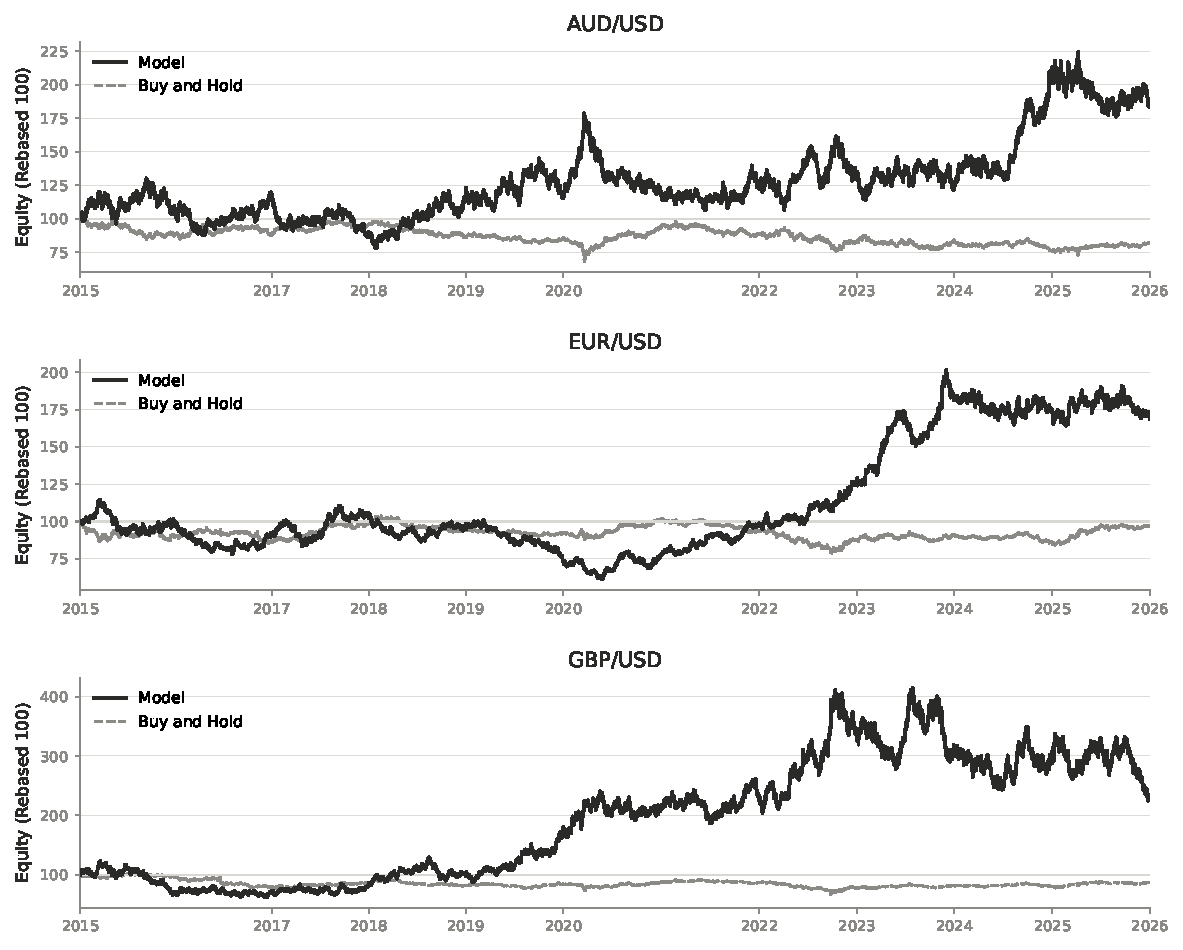
\includegraphics[width=\textwidth]{Images/PairEquityA.pdf}
\caption{AUD/USD, EUR/USD and GBP/USD against buying and holding the same pair, rebased to 100. All three benchmarks finish below their starting level.}
\label{Figure:PairEquityA}
\end{figure}

\subsubsection{EUR/USD}

EUR/USD is the cleanest demonstration in this work of return that is not market exposure. The pair finished almost exactly where it started, down $2.9\%$ across eleven years, and the agent returned $+70.6\%$. Its beta is $+0.266$ and its market exposure contributes $0.01$ percentage points per year, so of a $6.63\%$ mean yearly return, $6.62$ points are attributable to the policy. There was no trend to ride; the return came from timing alone.

It trades the shortest holding period of the seven, a median of $3.9$ days, at a modest $0.40$ of reference size, and its exposure is close to balanced at $55.5\%$ long across $1\,778$ positions. It won $51.9\%$ of them. Gross profit of $8\,734$ euros became $7\,064$ after $1\,669$ euros of commission, a $19.1\%$ share.

The equity curve, in Figure~\ref{Figure:PairEquityA}, shows why the headline figure needs qualifying in a different way from AUD/USD. Only five of eleven years are positive. The agent is roughly flat for the first six years of the window and produces almost all of its return between 2021 and 2023, when the pair moved in unusually wide ranges: $+27.3\%$, $+29.0\%$ and $+44.0\%$ in those three years, against $-25.3\%$ in 2019. This is a policy that needs volatility to work, and its maximum drawdown of $46.8\%$ reflects the periods when it did not get it.

\subsubsection{GBP/USD}

GBP/USD produced the highest alpha in the set at $+11.64\%$ per year, and it did so with a beta of $-0.054$ that is indistinguishable from zero. Its mean yearly return is $11.70\%$, of which $0.06$ points come from market exposure: as close to pure policy as any result here. Sterling itself fell $13.5\%$ over the window, so the agent's $+129.1\%$ sits $142.5$ percentage points above the benchmark.

It is the most active model, $2\,516$ positions, and also holds them the longest among the six working agents at a median of $12.6$ days, which means it runs many positions concurrently rather than trading quickly. It operates near full size at $0.89$ and wins $51.3\%$ of the time. Gross profit was $16\,630$ euros against $3\,168$ of commission, keeping $13\,462$.

Its returns concentrate in the years when sterling moved violently, which is visible in Figure~\ref{Figure:PairEquityA} as two steep sections: $+82.2\%$ in 2019 and $+52.0\%$ in 2022. Section~\ref{Subsection:TradingBehaviour} examines the second of those in detail. The same aggression produces the largest single losing year in the set, $-31.6\%$ in 2015, and the deepest drawdown, $50.4\%$. Seven of eleven years are positive. This is the most volatile of the profitable models and a reader should weigh its alpha against a drawdown that halved the account.

\subsubsection{NZD/USD}

The New Zealand Dollar fell furthest of the seven, $26.1\%$ over the window, and the agent returned $+60.1\%$ against it, an excess of $86.1$ points. Like AUD/USD it worked mostly from the short side, $24.0\%$ of positions long, with a beta of $-0.708$.

Its alpha of $+2.79\%$ per year is the smallest among the six profitable models, and with $1.83$ points of beta return in a $4.62\%$ mean return, a substantial minority of what it earned came from the market falling rather than from timing. On the alpha and beta reading it is the weakest of the six that worked.

Figure~\ref{Figure:PairEquityB} shows it alongside USD/CAD and USD/CHF. What distinguishes it is restraint, and the risk numbers reward it. It takes the fewest positions of the active models, $1\,011$, holds an average of $0.24$ of reference size, and produces a maximum drawdown of $23.3\%$, the second lowest in the set. Its Calmar ratio of $0.187$ is better than four pairs that returned considerably more, which is the point of measuring return against drawdown rather than in isolation. Gross profit was $7\,314$ euros and commission $1\,424$, a $19.5\%$ share. Seven of eleven years are positive, the best 2022 at $+14.5\%$ and the worst 2016 at $-6.4\%$; this is the steadiest of the moderately-sized models.

\begin{figure}[htb!]
\centering
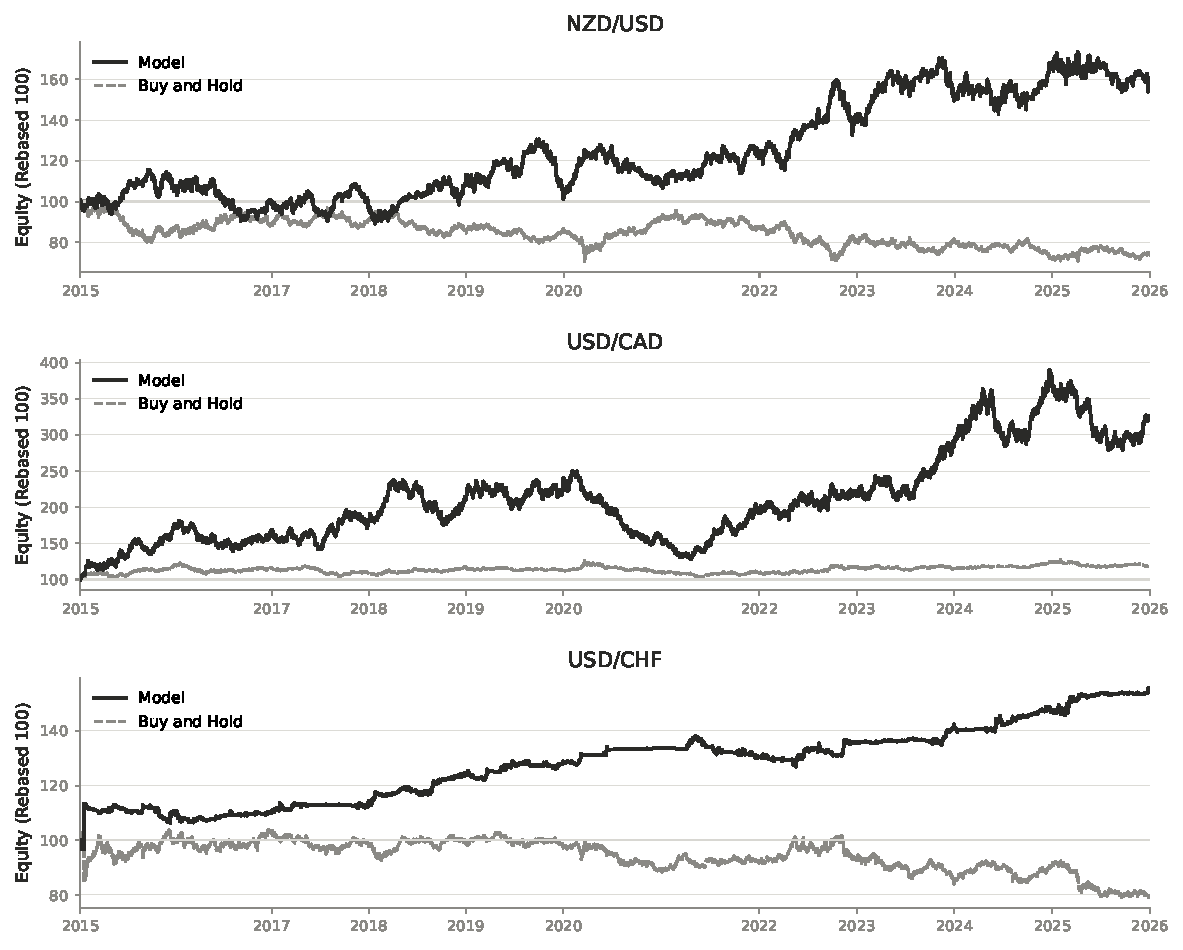
\includegraphics[width=\textwidth]{Images/PairEquityB.pdf}
\caption{NZD/USD, USD/CAD and USD/CHF against buying and holding the same pair, rebased to 100. USD/CAD is the only one of the three whose benchmark rises.}
\label{Figure:PairEquityB}
\end{figure}

\subsubsection{USD/CAD}

USD/CAD returned $+226.6\%$, by a wide margin the largest total in this work, and it is also the result that requires the most careful reading. Its beta of $+2.393$ is the highest of the seven and the pair itself rose $18.1\%$, so the agent was carrying a rising market at more than twice its size. Of a $14.23\%$ mean yearly return, $4.21$ points are beta return and $10.02$ are alpha.

That alpha is real and it is the second highest in the set, so this is not a model that merely looks good because its market went up. But leverage is symmetric, and the year-by-year record shows both sides of it: $+71.7\%$ in 2015, its best year and $52.7$ points clear of the benchmark, against $-34.8\%$ in 2020, its worst. Its maximum drawdown is $49.1\%$, and recovering from a $49\%$ drawdown requires a $96\%$ gain. Eight of eleven years are positive.

It is the second most active model at $2\,213$ positions with a median hold of $5.7$ days, runs at $0.79$ of reference size, and has the highest win rate in the set at $55.0\%$. It also earned the most in absolute terms, $25\,577$ euros gross, and paid $3\,432$ in commission for a $13.4\%$ share, lower than the four pairs above it because its profit per position was larger.

\subsubsection{USD/CHF}

USD/CHF returned $+54.8\%$, fifth of seven on return and first on every measure that accounts for risk. Its Sharpe ratio of $0.802$, Sortino of $1.552$ and Calmar of $0.492$ are the highest here, and its maximum drawdown of $8.2\%$ is a sixth of the worst. The Swiss Franc strengthened over the period so the pair fell $20.3\%$, and with a beta of $-0.082$ the agent took essentially none of that movement: of a $4.07\%$ mean yearly return, $3.91$ points are alpha.

Its behaviour explains every one of those numbers. It takes $220$ positions in eleven years, roughly one every eighteen days, and holds an average of $0.09$ of its reference size, a tenth of what it is permitted. Because it trades so little it pays almost nothing to trade: $130$ euros of commission against $5\,587$ of gross profit, a $2.3\%$ share where the set average is $16.0\%$. It keeps $97.7\%$ of what it earns while AUD/USD keeps $79.4\%$.

It is positive in ten of eleven years, the most consistent record in this work, with a worst year of $-2.4\%$. Its win rate of $49.8\%$ is the lowest of the seven, which is worth pausing on: the best model in the set is wrong slightly more often than a coin, and is the best anyway because of how it sizes and holds the positions it gets right. It is also the only model that made money in the held-out year of Section~\ref{Subsection:OutOfSample}. On return alone it would have placed fifth and been passed over; the selection criteria of Section~\ref{Subsection:ExperimentalProcedure} exist to prevent exactly that.

\subsubsection{USD/JPY}

USD/JPY is the failure of the set, and it is the only pair whose benchmark rose substantially. The pair gained $30.7\%$ over the window while the agent returned $+15.7\%$, finishing $14.4$ percentage points behind an investor who bought it and did nothing. Its beta of $+1.012$ and correlation of $+0.946$ with the pair's own yearly move describe what it became: a long position with extra steps and extra costs. Its alpha is $-1.08\%$ per year, the only negative figure in Table~\ref{Tables:AlphaBeta}.

Every position it takes is long, its median holding period is measured in years rather than days, and its average action is $0.98$, meaning it holds essentially full size continuously and has stopped making a sizing decision at all. It earned $1\,761$ euros gross, the least of the seven, and paid $155$ in commission. Five of eleven years are positive.

\begin{figure}[htb!]
\centering
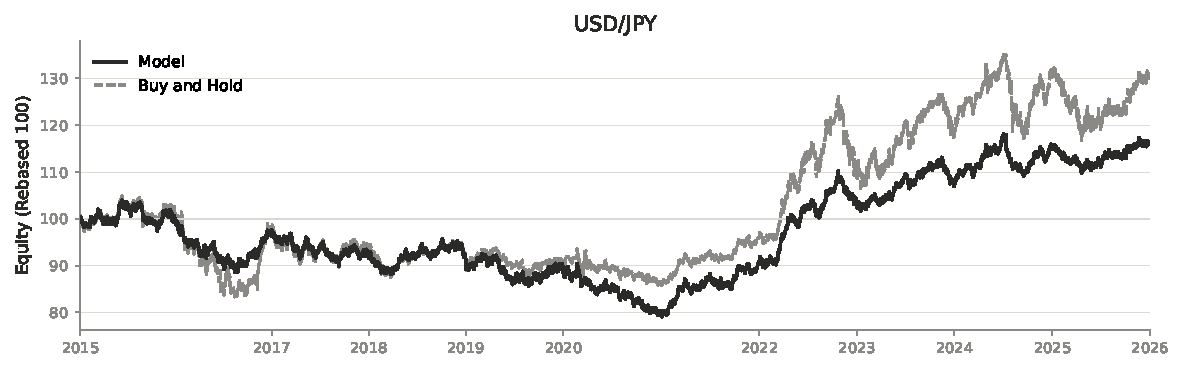
\includegraphics[width=\textwidth]{Images/PairEquityC.pdf}
\caption{USD/JPY against buying and holding the pair. The two lines track each other closely, which is the visual form of a beta of $+1.012$ and the reason this result is reported as a failure.}
\label{Figure:PairEquityC}
\end{figure}

Figure~\ref{Figure:PairEquityC} makes the point better than the statistics do: the model and the benchmark move together, with the model slightly below. Section~\ref{Subsection:NegativeResult} sets out the mechanism and what was tried against it.

\subsection{Trading Behaviour: How the Agents Actually Trade}
\label{Subsection:TradingBehaviour}

A return figure says whether an agent made money. It says nothing about how, and that matters here for a specific reason. The central claim of this work is that a continuous action lets one decision set both the direction and the size of a position. If the agents had learned to use only the extremes of that action, they would be discrete traders with extra machinery, and the claim would be empty. This subsection examines what they actually did.

\subsubsection{Use of the Continuous Action}

The agent emits an action $a \in [-1, 1]$ and holds $|a|$ of the reference size defined in Equation~\ref{Equation:PositionSizing}. Figure~\ref{Figure:ActionDistribution} shows how that value is distributed across the whole evaluation window for each pair.

\begin{table}[htb!]
\centering
\footnotesize
\begin{tabular}{@{}lrrrrrr@{}}
\toprule
\textbf{Pair} & \textbf{Positions} & \textbf{Long} & \textbf{Median Hold} & \textbf{Longest Hold} & \textbf{Win Rate} & \textbf{Mean $|a|$} \\
\midrule
AUD/USD & 1,561 & 27.9\% & 9.7 d & 227 d & 52.7\% & 0.77 \\
EUR/USD & 1,778 & 55.5\% & 3.9 d & 43 d & 51.9\% & 0.40 \\
GBP/USD & 2,516 & 46.9\% & 12.6 d & 149 d & 51.3\% & 0.89 \\
NZD/USD & 1,011 & 24.0\% & 5.9 d & 119 d & 52.8\% & 0.24 \\
USD/CAD & 2,213 & 65.6\% & 5.7 d & 97 d & 55.0\% & 0.79 \\
USD/CHF & 220 & 34.2\% & 8.0 d & 345 d & 49.8\% & 0.09 \\
USD/JPY & 1,438 & 100.0\% & 2,120 d & 4,004 d & 50.7\% & 0.98 \\
\bottomrule
\end{tabular}
\caption{Trading behaviour over the evaluation window. Mean $|a|$ is the average absolute action, that is the average fraction of the reference position size held while in the market. Win rate is the share of closed positions with a positive net result after costs.}
\label{Tables:Behaviour}
\end{table}

\begin{figure}[htb!]
\centering
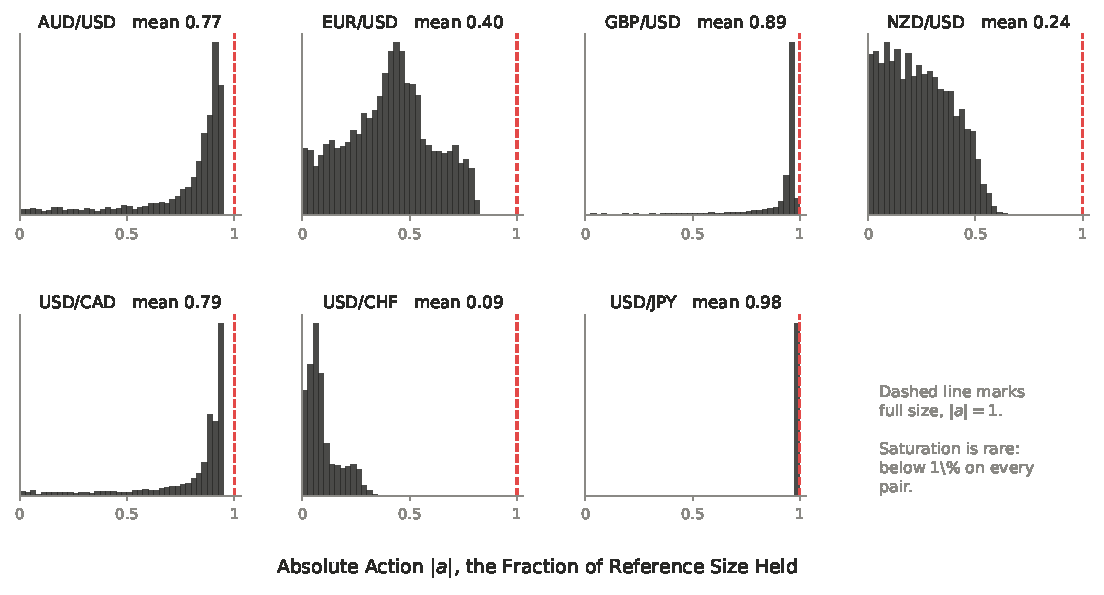
\includegraphics[width=\textwidth]{Images/ActionDistribution.pdf}
\caption{Distribution of the absolute action across the evaluation window. The dashed line marks full size. If the agents had reduced the continuous action to a discrete one, these histograms would be concentrated against that line; instead the mass sits across the interior of the range.}
\label{Figure:ActionDistribution}
\end{figure}

The action does not saturate. Fewer than one percent of decisions on any pair sit above $|a| = 0.98$, and on six of the seven pairs the figure is zero to one decimal place. The mean absolute action ranges from $0.09$ on USD/CHF to $0.98$ on USD/JPY, so the agents settled on very different operating sizes from the same design and the same reference risk.

That spread is itself informative. USD/CHF holds roughly a tenth of the size available to it, which is why its maximum drawdown is $8.2\%$ while its Sharpe ratio is the highest in the set: it found a small edge and sized it accordingly rather than pressing it. NZD/USD, at $0.24$, behaves similarly. USD/JPY sits at the opposite extreme with $0.98$, which is the numerical signature of the failure described in Section~\ref{Subsection:NegativeResult}: an agent that always holds full size in one direction has stopped making a sizing decision at all.

The sizing is adaptive in a second sense that the histogram does not show. The reference size itself is inversely proportional to the average true range, so a constant action produces a smaller position when volatility rises. The action and the volatility scaling compose, and the position actually held is the product of the two.

\subsubsection{Direction, Size and Outcome Together}

Figure~\ref{Figure:DecisionAnatomy} follows EUR/USD through three years, showing the price, the action the agent emitted, the position it held as a result, and the equity that followed.

\begin{figure}[htb!]
\centering
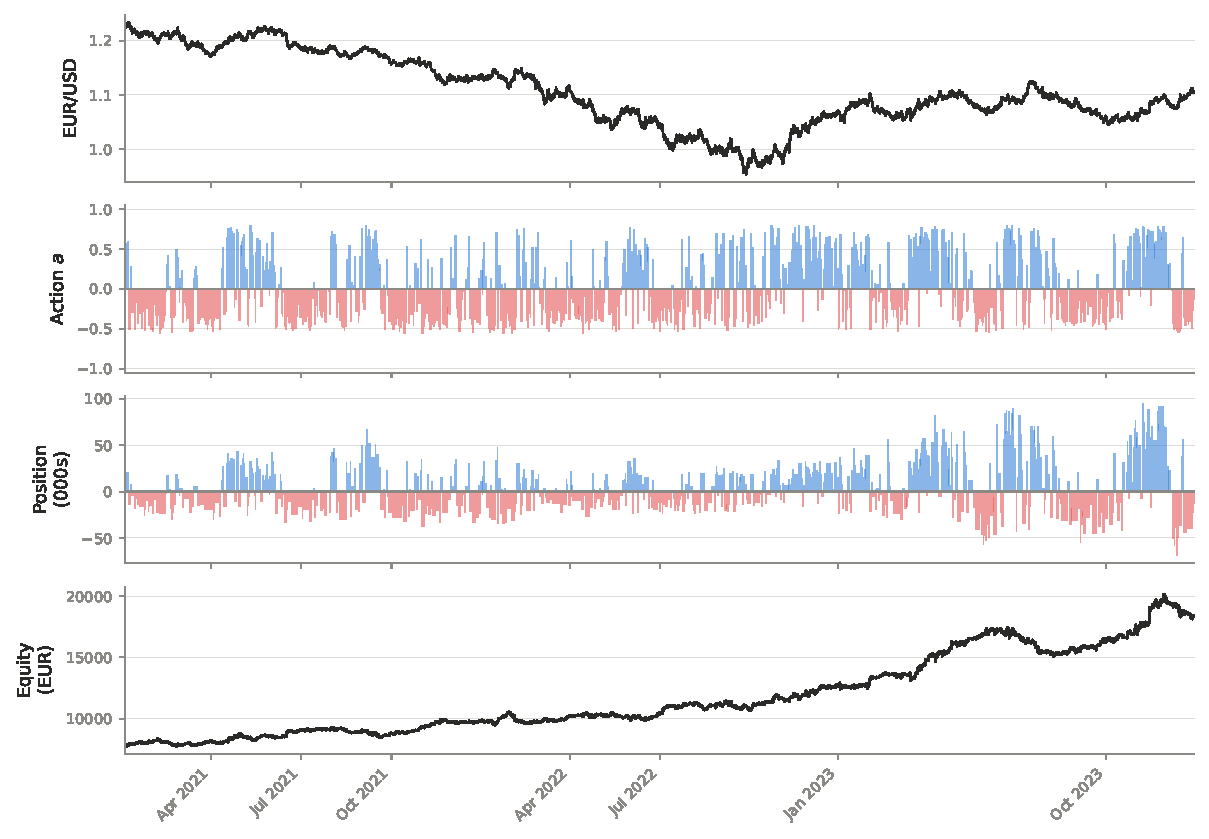
\includegraphics[width=\textwidth]{Images/DecisionAnatomy.pdf}
\caption{EUR/USD from 2021 to 2024. From top: the price; the action, positive for long and negative for short; the resulting net position in thousands of units; and account equity. The action changes sign well before the position does, because a change is only acted on when it exceeds the threshold of Equation~\ref{Equation:Hysteresis}.}
\label{Figure:DecisionAnatomy}
\end{figure}

Three behaviours are visible. The action moves continuously rather than switching between fixed levels, and its magnitude varies as much as its sign. The position follows the action but in coarser steps, because the rebalance threshold suppresses small adjustments; long stretches of constant position correspond to periods where the agent kept revising its target by less than the threshold. And the sign changes are not frequent: over a three-year window the agent reverses direction a few dozen times, which is consistent with the daily decision cadence rather than with an agent reacting to every bar it observes.

\subsubsection{Trend Identification and Reversal}

The clearest illustration of the agents holding a position through a sustained move is GBP/USD in the second half of 2022, shown in Figure~\ref{Figure:TrendRide}. Sterling fell from $1.22$ to below $1.04$ over roughly ten weeks, a decline of more than fifteen percent, with the sharpest part following the United Kingdom fiscal announcement of late September.

\begin{figure}[htb!]
\centering
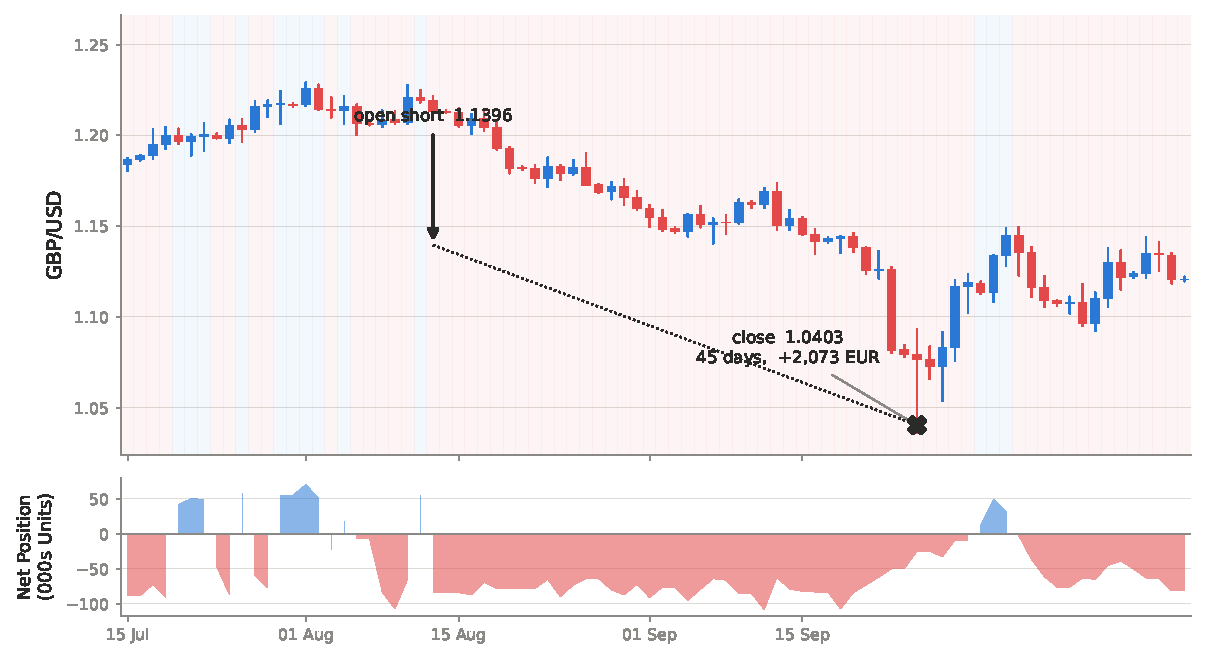
\includegraphics[width=\textwidth]{Images/TrendRide.pdf}
\caption{GBP/USD from mid-July to mid-October 2022. Background shading marks the direction of the net position, red for short and blue for long. The lower pane gives the size of that position. The annotated trade is the single most profitable position of the eleven years on this pair.}
\label{Figure:TrendRide}
\end{figure}

The agent was short for almost the entire decline. It held short exposure of between fifty and one hundred thousand units through the fall, added to it as the move developed, and reduced it into the low. The annotated position was opened at $1.1396$ on 12 August and closed at $1.0403$ on 26 September, forty-five days later, for a net profit of $2\,073$ euros after costs. It is the largest single position of the eleven years on this pair.

Two details are worth pointing out because they show discrimination rather than luck. The agent was briefly long at the end of July, at the local high before the decline began, and it was long again in the days immediately after the bottom, both times at small size. It did not hold the short indefinitely. Once the price recovered above $1.12$ in early October the position was reduced and then reversed, which is the behaviour of an agent responding to the state it observes rather than one committed to a direction.

\subsubsection{Holding Periods and Two-Sided Exposure}

Table~\ref{Tables:Behaviour} gives the trading statistics for each pair and Figure~\ref{Figure:HoldingBehaviour} shows two of them directly. Median holding periods run from four days on EUR/USD to nearly thirteen on GBP/USD, with the longest individual positions measured in months. These are swing traders, not scalpers, which is what the daily decision cadence of Section~\ref{Subsection:ExperimentalProcedure} was intended to produce.

\begin{figure}[htb!]
\centering
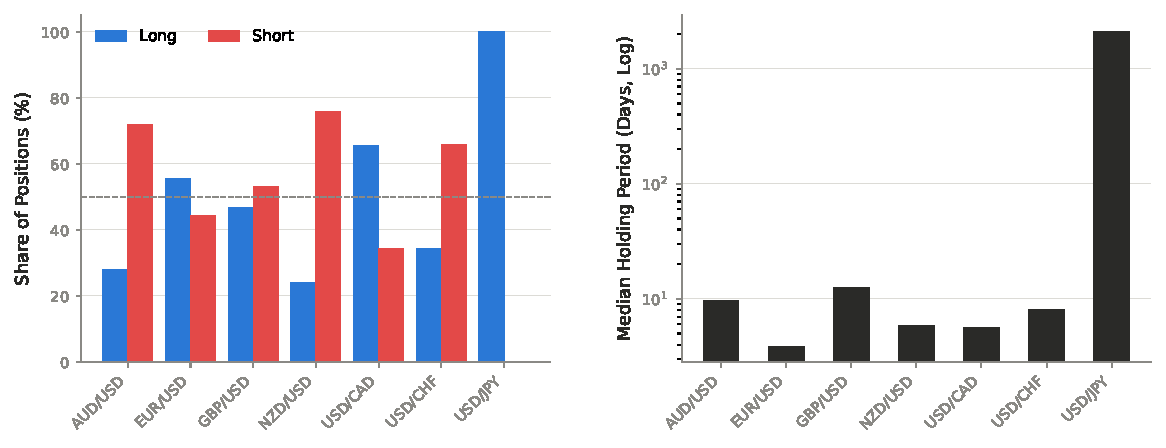
\includegraphics[width=\textwidth]{Images/HoldingBehaviour.pdf}
\caption{Left: the share of positions taken long and short. Right: the median holding period in days, on a logarithmic scale. USD/JPY is long in every position it takes and holds for years, which places it off the scale of the other six.}
\label{Figure:HoldingBehaviour}
\end{figure}

The long and short shares differ substantially between pairs, from $24\%$ long on NZD/USD to $66\%$ on USD/CAD, with EUR/USD and GBP/USD close to balanced. None of the six working agents is one-sided, which is a consequence of the design rather than an accident: the eligibility test of Section~\ref{Subsection:ExperimentalProcedure} rejected any episode whose weaker side fell below a threshold, so a one-sided policy could not be selected however profitable it looked. USD/JPY is the exception at $100\%$ long, and it is the exception precisely because that gate could not be satisfied on that pair by any of the $448$ seeds that were tried.

\subsubsection{Where the Edge Comes From}

One statistic in Table~\ref{Tables:Behaviour} is worth isolating. The win rate, the fraction of positions closed at a profit, lies between $49.8\%$ and $55.0\%$ across the seven pairs. Six of the seven are within three points of a coin flip, and the best model in the set by every risk measure, USD/CHF, has the lowest win rate of all at $49.8\%$.

The agents are therefore not profitable because they are right more often than they are wrong. They are profitable because of what they do with a position once it is open: the size held when the position moves favourably is larger than the size held when it does not, and positions that work are held for longer than positions that do not. That is what a continuous action buys, and it is not available to an agent that can only choose a direction. It also explains why USD/CHF can be the strongest model in the set while being wrong slightly more often than a coin: it is small and patient, and the few positions it holds at size are the ones that worked.

\subsubsection{What the Trading Costs}

Because the engine charges the spread quoted at each fill and a real commission schedule, the difference between what the policies earned and what the account kept can be measured rather than estimated.

The commission is recorded directly on every trade. The spread is not, because it is paid inside each fill rather than deducted after it: a buy is filled at the ask and a sell at the bid, so the cost is already embedded in the entry and exit prices. It can nonetheless be recovered exactly, because the two charges scale in the same way. Commission is levied at $3.5$ points per side, seven points for a round turn, and the spread is crossed once per round turn. Both are proportional to the traded volume and both are converted into the account currency at the same rate, so for any position

\begin{equation}
C_{spread} = \left| C_{commission} \right| \cdot \frac{s}{7}
\label{Equation:SpreadRecovery}
\end{equation}

where $s$ is the spread in points at the moment of the trade. Applying Equation~\ref{Equation:SpreadRecovery} to every position, with $s$ taken from the recorded quotes for the month in which the position was opened, gives Table~\ref{Tables:Costs}.

\begin{table}[htb!]
\centering
\footnotesize
\begin{tabular}{@{}lrrrrrr@{}}
\toprule
\textbf{Pair} & \textbf{Before Costs} & \textbf{Spread} & \textbf{Commission} & \textbf{Net} & \textbf{Cost Share} & \textbf{Mean Spread} \\
\midrule
AUD/USD & 11,851 & $-1,162$ & $-2,200$ & 8,488 & 28.4\% & 3.70 pts \\
EUR/USD & 9,372 & $-638$ & $-1,669$ & 7,064 & 24.6\% & 2.68 pts \\
GBP/USD & 19,086 & $-2,456$ & $-3,168$ & 13,462 & 29.5\% & 5.43 pts \\
NZD/USD & 8,552 & $-1,238$ & $-1,424$ & 5,890 & \textbf{31.1\%} & 6.09 pts \\
USD/CAD & 28,272 & $-2,695$ & $-3,432$ & 22,145 & 21.7\% & 5.50 pts \\
USD/CHF & 5,735 & $-148$ & $-130$ & 5,457 & \textbf{4.8\%} & 7.93 pts \\
USD/JPY & 2,172 & $-411$ & $-155$ & 1,606 & 26.1\% & 18.53 pts \\
\midrule
\textbf{Total} & \textbf{85,039} & $\mathbf{-8,748}$ & $\mathbf{-12,179}$ & \textbf{64,112} & \textbf{24.6\%} & --- \\
\bottomrule
\end{tabular}
\caption{What the seven agents earned before costs and what they kept, in euros. Cost share is the spread and commission together as a fraction of profit before costs. The mean spread column is the commission-weighted average spread paid, in points, which differs from the pair's average spread because it weights the moments the agent actually traded.}
\label{Tables:Costs}
\end{table}

The seven agents earned $85\,039$ euros before costs and kept $64\,112$. Of the difference, $8\,748$ euros went to the spread and $12\,179$ to commission, so \textbf{costs consumed $24.6\%$ of trading profit}. Commission is the larger of the two charges here, which is a consequence of trading a raw-spread account: the spread is narrow by design and the broker recovers its margin explicitly instead. On an account quoting wider spreads with no commission, the same trades would have paid a similar total in a different proportion.

The swap column is absent from Table~\ref{Tables:Costs} because it is zero on every pair. On a swap-free account no overnight financing is charged, so that is the exact figure rather than an approximation, and it matters at this holding horizon: agents holding positions for a median of four to thirteen days would otherwise pay financing on several hundred nights each.

The variation between pairs follows turnover almost exactly, and it is large. USD/CHF takes $220$ positions and surrenders $4.8\%$ of its pre-cost profit, keeping more than nineteen euros in twenty. NZD/USD surrenders $31.1\%$ and GBP/USD $29.5\%$. The same quality of policy therefore delivers very different net results at different trading frequencies, which is why the selection criteria of Section~\ref{Subsection:ExperimentalProcedure} reward long holding periods directly rather than trusting the return figure to account for them, and why the rebalance threshold of Equation~\ref{Equation:Hysteresis} contributes as much as Table~\ref{Tables:Deployment} indicates.

One consequence deserves emphasis because it bears on how the rest of this section should be read. Every return quoted in this work is net of both charges. A study reporting the same policies on bar closes with no spread and no commission would have reported the pre-cost column of Table~\ref{Tables:Costs}, which is a third larger, and it would have been describing a strategy that no account could have traded.

Recovering the spread through Equation~\ref{Equation:SpreadRecovery} works but is indirect, and it relies on the commission being non-zero. The engine computes the spread charge internally when it opens a position and does not currently carry it into the exported trade record as its own field. Recording it there, alongside commission and swap, is a straightforward improvement and is noted in Section~\ref{Subsection:FutureWork}.

\subsection{Path Robustness}

Each pair was evaluated from the five starting balances of Section~\ref{Subsection:EvaluationProtocol}. The result is the same in every case: all seven pairs are profitable from all five entry points, thirty-five runs in total, with no exceptions.

The spread across the five is small relative to the returns themselves. The relative standard deviation, the standard deviation divided by the mean, runs between $4\%$ and $10\%$ across the seven pairs. USD/JPY is the tightest at $4.4\%$ and GBP/USD the widest at $10.4\%$ in absolute terms, though as a fraction of a much larger return it is the smaller effect.

This matters because of how position sizes are computed. A volume is rounded to the broker's step, so a starting balance a hundred euros higher can round a position differently, which changes the equity available for the next position and eventually the entire sequence of trades. Two runs that differ only in their opening balance are therefore not the same run with a scale factor; they are different sequences. That all thirty-five are profitable says the results do not depend on one particular path through the data.

What this protocol does not measure is the variation between training runs. Each published model is one seed drawn from a pool of $128$ to $256$, and the spread across that pool is a separate question, addressed in Section~\ref{Subsection:StatisticalScreening}.

\subsection{Alpha and Beta Decomposition}
\label{Subsection:AlphaBeta}

A currency pair moves on its own. An agent that is long a pair which happens to rise will show a profit that has nothing to do with the policy it learned, and an agent that is short a pair which happens to fall will show the same. Total return cannot tell the two apart, so the results are decomposed into the part explained by the market and the part that is not.

For each pair the yearly return of the model is regressed on the yearly move of the pair itself, over the eleven years from 2015 to 2025. Writing $r_i$ for the model return in year $i$ and $m_i$ for the market move in the same year, ordinary least squares gives

\begin{equation}
\beta = \frac{\sum_i (m_i - \bar{m})(r_i - \bar{r})}{\sum_i (m_i - \bar{m})^2}, \qquad \alpha = \bar{r} - \beta \bar{m}
\label{Equation:AlphaBeta}
\end{equation}

$\beta$ is how much of the market's movement the model carries, and $\alpha$ is the average yearly return left once that exposure is removed. The mean return then splits into an active part and a passive one:

\begin{equation}
\bar{r} = \underbrace{\alpha}_{\text{policy}} + \underbrace{\beta \bar{m}}_{\text{market exposure}}
\label{Equation:AlphaDecomposition}
\end{equation}

Yearly rather than daily returns are used for a specific reason. The agents hold positions for days to weeks and act once per day, so a daily regression would measure how the model tracks the market within a holding period rather than whether it chose the right direction over the horizon it trades. Eleven yearly observations is a small sample and the individual coefficients carry wide uncertainty; what the decomposition supports is the separation of pairs into groups, not a precise value for any one of them.

Table~\ref{Tables:AlphaBeta} gives both terms. Six of the seven pairs have positive alpha, and the seven fall into three clear groups.

\begin{table}[htb!]
\centering
\footnotesize
\begin{tabular}{@{}lrrrrl@{}}
\toprule
\textbf{Pair} & \textbf{Beta} & \textbf{Alpha (\%/yr)} & \textbf{Beta Return (\%/yr)} & \textbf{Mean (\%/yr)} & \textbf{Reading} \\
\midrule
AUD/USD & $-2.013$ & $+4.96$ & $+3.22$ & $+8.18$ & Policy plus leveraged trend \\
EUR/USD & $+0.266$ & $+6.62$ & $+0.01$ & $+6.63$ & Policy, no market exposure \\
GBP/USD & $-0.054$ & $+11.64$ & $+0.06$ & $+11.70$ & Policy, no market exposure \\
NZD/USD & $-0.708$ & $+2.79$ & $+1.83$ & $+4.62$ & Policy plus leveraged trend \\
USD/CAD & $+2.393$ & $+10.02$ & $+4.21$ & $+14.23$ & Policy plus leveraged trend \\
USD/CHF & $-0.082$ & $+3.91$ & $+0.16$ & $+4.07$ & Policy, no market exposure \\
USD/JPY & $+1.012$ & $-1.08$ & $+2.64$ & $+1.57$ & No policy; the model is the market \\
\bottomrule
\end{tabular}
\caption{Decomposition of Equation~\ref{Equation:AlphaDecomposition}, from the yearly regression of Equation~\ref{Equation:AlphaBeta} over 2015 to 2025. Alpha is the return attributable to the policy and the beta return is the part explained by the pair's own movement. The two sum to the mean yearly return.}
\label{Tables:AlphaBeta}
\end{table}

\textbf{Three pairs carry almost no market exposure.} GBP/USD, EUR/USD and USD/CHF have betas of $-0.054$, $+0.266$ and $-0.082$, and their market exposure contributes $0.06$, $0.01$ and $0.16$ percentage points per year respectively. For GBP/USD, $11.64$ of its $11.70$ points per year are policy. These are the results that would survive a change in market direction, because there is almost no direction in them to change.

\textbf{Three pairs combine policy with leveraged exposure.} USD/CAD at $+2.393$, AUD/USD at $-2.013$ and NZD/USD at $-0.708$ all carry their market at meaningful size, two of them at more than twice. Their alpha is positive in every case, so there is skill on top, but between a fifth and two fifths of what they earned came from the market moving the way their exposure was pointed. USD/CAD is the clearest example: $4.21$ of its $14.23$ points per year came from the pair rising while the agent was net long. Had the Canadian Dollar strengthened over the decade instead, that component would have been a loss of similar size, and the reported $+226.6\%$ would look very different.

Figure~\ref{Figure:AlphaBeta} plots the seven together, and the three groups separate clearly.

\textbf{One pair has no policy at all.} USD/JPY has a beta of $+1.012$ and a correlation of $+0.946$ with its own market, and its alpha is $-1.08\%$ per year, the only negative figure in the table. It is examined in Section~\ref{Subsection:NegativeResult}.

\begin{figure}[htb!]
\centering
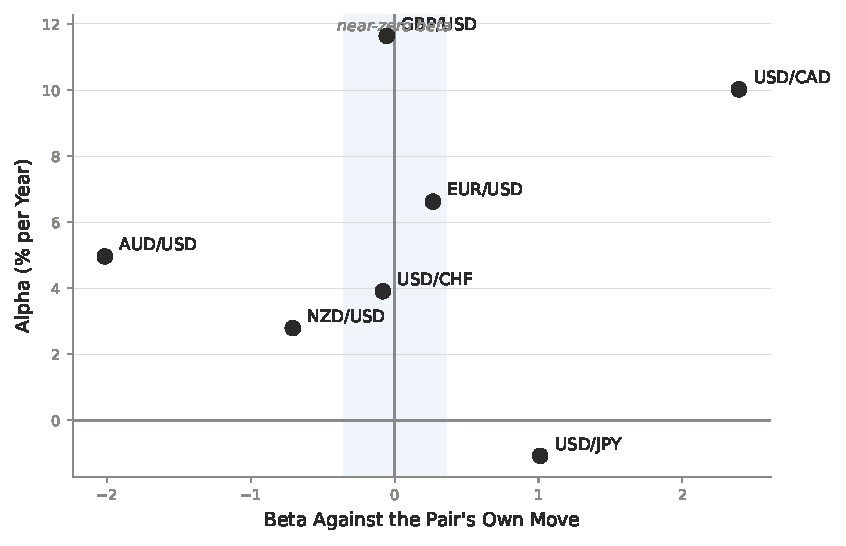
\includegraphics[width=0.82\textwidth]{Images/AlphaBeta.pdf}
\caption{Alpha against beta for the seven agents. Points inside the shaded band carry almost no market exposure, so their return is attributable to the policy. USD/JPY sits at a beta of one with negative alpha, which is the signature of a model that has reproduced its own market.}
\label{Figure:AlphaBeta}
\end{figure}

The method was checked before it was applied. Running the same regression on the model delivered by the preceding campaign reproduces its recorded figures exactly, a correlation of $+0.115$, a beta of $+0.130$ and an alpha of $+3.11\%$ per year, which confirms that the decomposition here is computed the same way as the one it is compared against.

This decomposition is reported ahead of total return for a reason that matters to how the whole section should be read. The choice of which model to publish was made from a pool of candidates, and any measure that the choice was made on is inflated by that choice. Return is such a measure. Beta is not: it describes how a policy behaves against its market, and a model cannot be selected into a low beta by luck in the way it can be selected into a high return. A large alpha with a beta near zero is therefore a stronger claim than a large return, and it is the claim this work leads with.

\subsection{Statistical Screening and the Rejected Candidates}
\label{Subsection:StatisticalScreening}

Every published model had to pass a test against a null built from itself. The model's own sequence of positions is rotated in time, so that it holds the same positions for the same durations but at the wrong moments, and the resulting regime score is the score its holding structure earns by luck alone. The published model must beat that score.

The null has to be computed per model rather than fixed. Measured across the seven pairs it ranges from $48.21$ on GBP/USD to $69.82$ on NZD/USD. A fixed threshold of, say, $55$ would sit below chance on one pair and well above it on another, so it would accept noise in one market and reject skill in another. This was found by trying the fixed threshold first.

The screening produced a result that changes how the whole campaign should be read. \textbf{In every one of the seven pairs, the candidate with the highest return failed the test.} Table~\ref{Tables:BetaTraps} lists the strongest cases. A portfolio built by ranking candidates on return would have selected models averaging roughly $+250\%$, almost all of which is market exposure rather than policy.

\begin{table}[htb!]
\centering
\footnotesize
\begin{tabularx}{\textwidth}{@{}lrrX@{}}
\toprule
\textbf{Pair} & \textbf{Return} & \textbf{$p$-value} & \textbf{Why it was rejected} \\
\midrule
AUD/USD & $+246.8\%$ & $0.146$ & Failed the screen \\
AUD/USD & $+142.6\%$ & $0.987$ & Published during the campaign, then withdrawn when the test was run \\
EUR/USD & $+141.6\%$ & --- & One-sided: long for $86\%$ of the window \\
GBP/USD & $+259.8\%$ & $0.163$ & Failed the screen \\
NZD/USD & $+253.9\%$ & $0.258$ & Failed the screen \\
USD/CHF & $+463.9\%$ & $0.973$ & Positions no better timed than the same positions shuffled; rode the franc trend \\
USD/CHF & $+341.3\%$ & $0.865$ & As above \\
\bottomrule
\end{tabularx}
\caption{Candidates rejected by the screening of Section~\ref{Subsection:StatisticalScreening}. In every pair the highest-return candidate failed. Ranking on return alone would have selected these models over the ones published, at roughly five times the apparent return and almost none of the measurable skill.}
\label{Tables:BetaTraps}
\end{table}

The USD/CHF case is the clearest. A candidate returning $+463.94\%$, more than nine times the published model, has a permutation $p$-value of $0.973$: its positions are no better timed than the same positions shuffled. It rode the franc's trend. The published model returns a ninth of that and is the one with measurable skill.

Two cases are worth reporting because they are uncomfortable. An AUD/USD candidate returning $+142.55\%$ was published during the campaign and then withdrawn when its $p$-value came out at $0.987$. And on EUR/USD the incumbent model won on four of six metrics, including return, Sharpe, Sortino and drawdown, and was still replaced, because it lost on the one axis that decides whether a result is real.

The limits of this screening should be stated. Each published model was chosen from between $128$ and $256$ candidates, so a $p$-value near $0.05$ is close to what that many draws produce by chance. Under a strict correction for the number of candidates examined, only USD/CAD and GBP/USD, both at $0.0015$, would clearly survive. The permutation test is therefore used here as a screen that rejected bad models, which it demonstrably did, and not as a claim of statistical significance for the ones that remain.

\subsection{Out-of-Sample Behaviour: The Held-Out Year}
\label{Subsection:OutOfSample}

The split of Equation~\ref{Equation:Split} trains on 2015 to 2023, selects among episodes on 2024, and leaves 2025 untouched. Because the trained weights are stored, 2025 can be scored on its own.

\textbf{It is negative.} Table~\ref{Tables:TestYear} gives the figures: five of the seven pairs lose money in 2025, and the mean model return is $-6.8\%$ against a mean market move that would have made money. Only USD/CHF, at $+5.0\%$, and USD/JPY, at $+0.6\%$, are positive.

\begin{table}[htb!]
\centering
\footnotesize
\begin{tabular}{@{}lrrrr@{}}
\toprule
\textbf{Pair} & \textbf{2025 (Test)} & \textbf{2024 (Validation)} & \textbf{Full Window} & \textbf{2025 Market} \\
\midrule
AUD/USD & $-11.7\%$ & $+72.4\%$ & $+102.5\%$ & $+7.6\%$ \\
EUR/USD & $-1.2\%$ & $-5.9\%$ & $+73.9\%$ & $+13.5\%$ \\
GBP/USD & $-22.9\%$ & $-3.6\%$ & $+124.1\%$ & $+7.6\%$ \\
NZD/USD & $-5.0\%$ & $+11.0\%$ & $+56.4\%$ & $+2.8\%$ \\
USD/CAD & $-13.4\%$ & $+28.8\%$ & $+226.6\%$ & $-4.6\%$ \\
USD/CHF & $\mathbf{+5.0\%}$ & $+3.7\%$ & $+50.6\%$ & $-12.8\%$ \\
USD/JPY & $+0.6\%$ & $+7.6\%$ & $+15.7\%$ & $-0.7\%$ \\
\midrule
\textbf{Portfolio} & $\mathbf{-9.8\%}$ & --- & $+91.3\%$ & --- \\
\bottomrule
\end{tabular}
\caption{The held-out year against the validation year and the full window. 2025 was seen by no part of the training or selection procedure; 2024 was used to choose which episode's weights were kept. The last column is the move of the pair itself in 2025.}
\label{Tables:TestYear}
\end{table}

The contrast with 2024 is the important part, and Figure~\ref{Figure:YearlyExcess} shows it directly. 2024 is the best year in the whole sample, with a mean excess return over the benchmark of $+16.4$ percentage points. 2025 is the worst, at $-8.7$. The difference between those two years is that 2024 was used to decide which episode's weights were kept and 2025 was used for nothing. That is what selection pressure looks like when it is measured, and it is the reason the full-window figures in Table~\ref{Tables:PairResults} are described as an in-sample result throughout this document.

\begin{figure}[htb!]
\centering
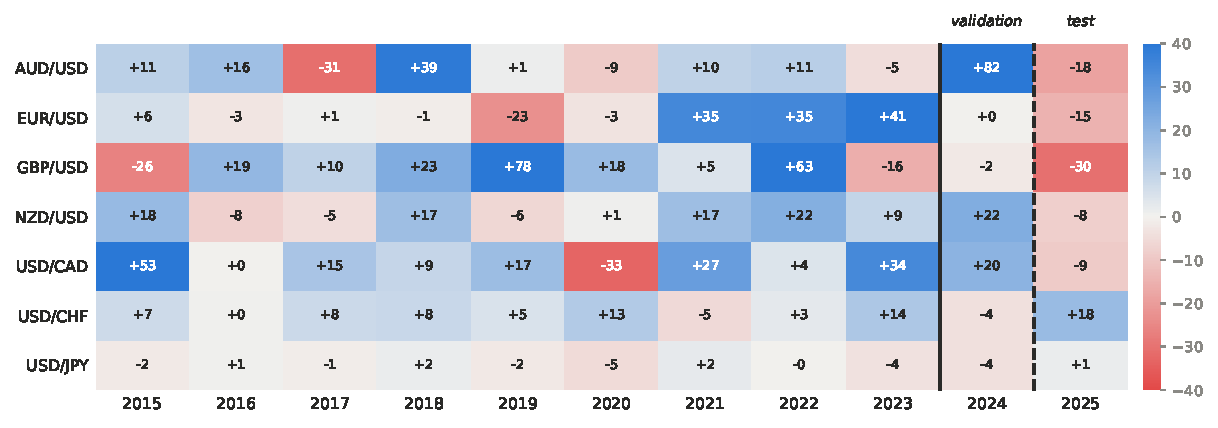
\includegraphics[width=\textwidth]{Images/YearlyExcess.pdf}
\caption{Yearly return of each agent minus the return of buying and holding the same pair, in percentage points. Blue is outperformance. The solid line marks the end of the training data and the dashed line the end of the validation year, so only the last column was unseen by any part of the procedure.}
\label{Figure:YearlyExcess}
\end{figure}

There is a market explanation for the direction of the 2025 result, and it is worth giving because it points somewhere. 2025 was a broad dollar reversal: EUR/USD rose $13.5\%$, its largest annual move in the eleven years, and the dollar weakened against five of the seven pairs. The agents were trained on a decade in which the dollar mostly strengthened, and six of the seven were positioned for that. The seventh, USD/CHF, is the least directional model in the set, holds the fewest positions and has the lowest beta, and it is the one that made money. That is consistent with the rest of the evidence rather than a coincidence: the model that depends least on a market direction is the one that survived the direction changing.

The individual results are worth reading rather than only their average, because they do not fail in the same way. GBP/USD is the worst at $-22.9\%$, and it is the most aggressive model in the set, running near full size with the deepest drawdown over the full window; a year that goes against it costs accordingly. USD/CAD loses $13.4\%$ and AUD/USD $11.7\%$, and both are the leveraged-exposure models of Section~\ref{Subsection:AlphaBeta}, so a reversal in the direction their beta points is exactly the event that hurts them. EUR/USD loses only $1.2\%$ despite the pair moving $13.5\%$, which is consistent with its near-zero beta: it did not participate in the reversal in either direction.

The two that held up are the two that were holding least. USD/CHF returned $+5.0\%$ while its pair fell $12.8\%$, an excess of $17.8$ percentage points and its best year against the benchmark in the whole sample. USD/JPY returned $+0.6\%$, which is not skill but the absence of exposure to the pairs that moved. Between them they describe the pattern: the models that depended least on a market direction were the ones that survived the direction changing.

One year is a small sample and no conclusion should be drawn from it beyond the obvious one. What the held-out year establishes is a bound, not a verdict: the design continued to trade sensibly on data it had never seen, and it lost money doing so in a year whose direction its training data did not contain.

\subsection{A Negative Result: USD/JPY}
\label{Subsection:NegativeResult}

USD/JPY did not work, and the reason is understood.

The numbers say the model is the market. Its correlation with the pair's yearly move is $+0.946$ and its beta is $+1.012$, so it carries the pair almost exactly one for one. Its alpha is $-1.07\%$ per year. It returns $+15.7\%$ over the eleven years against roughly $+25\%$ for simply buying and holding the pair, so it underperforms the benchmark that costs nothing to run. The model is long at every point in the window.

The mechanism is in the data. USD/JPY rose from roughly $120$ to $150$ over the period, with the move concentrated and largely one-directional. On such a series, holding a long position is close to optimal, and any deviation from it is punished. The reward signal therefore offers no gradient towards modulating exposure, and the agent settles on the simplest policy that captures the trend. The other six majors mean-revert enough over the same period that two-sided behaviour is rewarded, and their agents learned it.

This was tested rather than assumed. Across seven configurations and $448$ seeds, every run converged to an all-in directional policy. Raising the augmentation that presents the agent with mirrored price series, which was intended to remove exactly this bias, made the resulting policies more binary rather than less.

The result is reported because it is informative. It marks the boundary of the method: this design learns to time exposure in markets that turn, and on a market that does not turn it reduces to holding the trend and pays costs for the privilege. A reader deciding whether to apply the approach elsewhere needs that boundary more than they need a seventh success.

\subsection{Portfolio: The Seven Models Combined}
\label{Subsection:Portfolio}

A trader would not run one of these agents. They would run all seven, which is a different question from how each performs alone, because what matters for a portfolio is not only what each component returns but whether they lose money at the same time.

The seven published models are combined by giving each a seventh of the capital at the start of the window and never rebalancing. Writing $E_p(t)$ for the equity of pair $p$ at time $t$, the portfolio is

\begin{equation}
V(t) = \frac{1}{7} \sum_{p} \frac{E_p(t)}{E_p(0)}
\label{Equation:Portfolio}
\end{equation}

The total return of such a portfolio is the mean of its components by construction, so the return is not the interesting part. The risk is. Table~\ref{Tables:Portfolio} sets the portfolio against the average of the seven pairs taken separately.

\begin{table}[htb!]
\centering
\footnotesize
\begin{tabular}{@{}lrrl@{}}
\toprule
\textbf{Measure} & \textbf{Portfolio} & \textbf{Mean of the seven} & \textbf{Effect} \\
\midrule
Total return & $+91.3\%$ & $+91.3\%$ & Equal by construction \\
Annualised return & $+6.07\%$ & $+6.07\%$ & Equal by construction \\
\addlinespace
Maximum drawdown & $\mathbf{15.9\%}$ & $34.5\%$ & More than halved \\
Sharpe ratio & $\mathbf{0.632}$ & $0.451$ & Above all but USD/CHF \\
Sortino ratio & $0.906$ & $0.685$ & Improved \\
Calmar ratio & $0.381$ & $0.194$ & Nearly doubled \\
Sterling ratio & $1.059$ & $0.670$ & Improved \\
\addlinespace
Mean correlation & \multicolumn{2}{c}{$+0.062$ across all 21 pairings} & Near independence \\
\bottomrule
\end{tabular}
\caption{The equal-weight portfolio of Equation~\ref{Equation:Portfolio} against the average of its seven components. Return is identical by construction, so the whole effect is on risk.}
\label{Tables:Portfolio}
\end{table}

The maximum drawdown falls from an average of $34.5\%$ to $15.9\%$, and the Sharpe ratio rises from an average of $0.451$ to $0.632$, above every individual pair except USD/CHF. The same return is delivered with less than half the worst loss.

\begin{figure}[htb!]
\centering
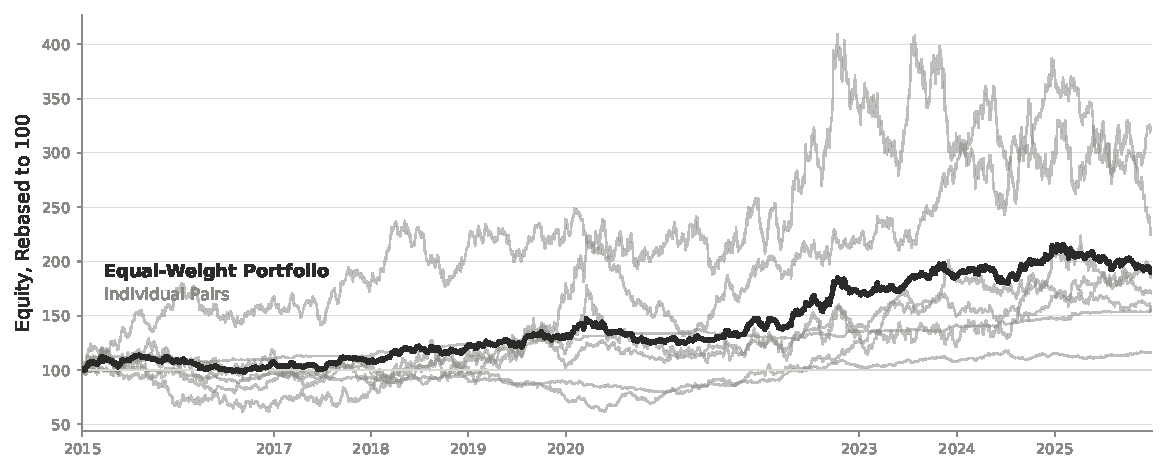
\includegraphics[width=\textwidth]{Images/PortfolioEquity.pdf}
\caption{The equal-weight portfolio against its seven components, all rebased to 100. The portfolio is smoother than any component because the components do not fall together.}
\label{Figure:PortfolioEquity}
\end{figure}

The reason is in Figure~\ref{Figure:Correlation}. The mean correlation between the daily returns of any two of the seven models is $+0.062$, and no pair of models exceeds $+0.46$. Three pairings are negative. These are seven agents trained by the same procedure on seven instruments that are themselves correlated, all sharing the US Dollar on one side, and yet their profits and losses arrive at different times. That is a consequence of the design: each agent learned the timing of its own market, so what they have in common is a method rather than a position.

\begin{figure}[htb!]
\centering
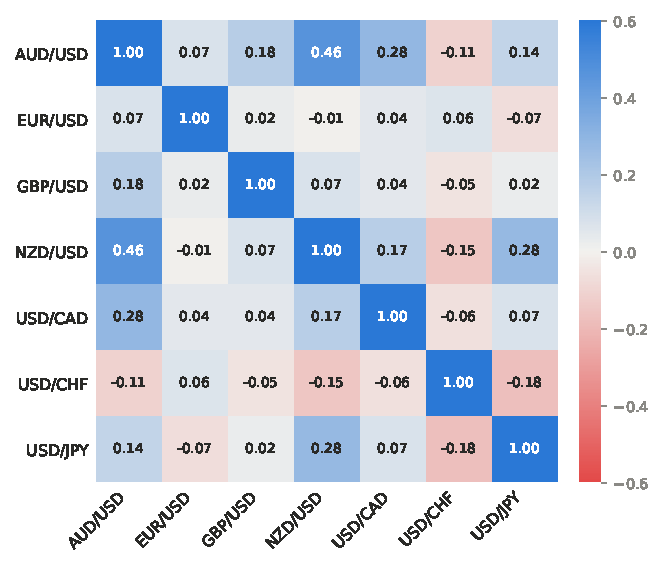
\includegraphics[width=0.68\textwidth]{Images/Correlation.pdf}
\caption{Correlation between the daily returns of the seven agents over the evaluation window. The mean of the off-diagonal entries is $+0.062$.}
\label{Figure:Correlation}
\end{figure}

Two qualifications belong with this result. The components do not all run at the same position size, as Section~\ref{Subsection:EvaluationProtocol} states, so the portfolio is the combination as published rather than a risk-parity allocation; equalising the sizes would change the weights but not the correlation structure that produces the benefit. And the portfolio inherits the limitation of its components: in the held-out year of Section~\ref{Subsection:OutOfSample} it returns $-9.8\%$, better than five of the seven pairs and worse than two, which is what an average should do when most of its components fall together for a reason they share.

Two results carry the most weight. Six of the seven agents produced positive alpha against their own market, and three of those did it with a market sensitivity close to zero, which is what separates a strategy from leveraged exposure. And the seven combined behave better than any of them alone, because they are close to uncorrelated.

Against that, the held-out year is negative and the selection is uncorrected. Section~\ref{Section:Conclusion} sets out what those two facts allow the work to claim and what they do not.